\documentclass[es]{uc3mreport}


\usepackage{import}

\usepackage{listings}  % package for code listings
\usepackage{float}     % for H placement specifier

\usepackage{mymacros}  % report-specific macros

% general config

\graphicspath{{img/}}  % Images folder
 \addbibresource{references.bib}  % bibliography file

\degree{Máster en Ingeniería Informática}
\subject{Aplicaciones Avanzadas de la Inteligencia Artificial}
\year{2024-2025}  % academic year
\group{1}
\author{
  Jorge Ramos Santana -- 100451001\\
  Luis Daniel Casais Mezquida -- 100429021\\
  Carlos Salinas Gancedo -- 100549334
}
 \team{Equipo 1}
\shortauthor{
  \abbreviateauthor{Jorge}{Ramos Santana},
  \abbreviateauthor{Luis Daniel}{Casais Mezquida} \& 
  \abbreviateauthor{Carlos}{Salinas Gancedo}
 }
\lab{Práctica 2}
\title{IA en la salud}
\professor{María Paula de Toledo}


\begin{document}
  \makecover[old]

  \tableofcontents
  \listoffigures
  % \listoftables

  % contenidos
  \begin{report}

    \section{Introducción y enfoque del problema}
    
    En esta práctica abordamos el desarrollo de un clasificador de imágenes de rayos X para la detección de COVID-19. El objetivo de nuestro trabajo es desarrollar un modelo de clasificación basado en deep learning capaz de diferenciar entre radiografías torácicas de pacientes con COVID-19 y pacientes sanos (normales). Para ello, utilizaremos técnicas redes neuronales convolucionales (CNN) que han demostrado un gran rendimiento en tareas similares de clasificación de imágenes médicas.
    
    \subsection{Antecedentes}
    
    Desde el inicio de la pandemia, numerosos grupos de investigación han explorado el uso de técnicas de deep learning para la detección de COVID-19 en imágenes médicas \cite{Tartaglione_2020} \cite{lara2025diagnosingcovid19severitychest}. Los enfoques basados en transfer learning con arquitecturas pre-entrenadas como ResNet, DenseNet o EfficientNet han sido ampliamente utilizados. Estos modelos aprovechan el conocimiento adquirido en grandes conjuntos de datos de imágenes generales y lo adaptan a la tarea específica de clasificación de radiografías.
    
    \section{Metodología}
    
    \subsection{Decisiones de diseño e implementación}
    
    Para el desarrollo de nuestro clasificador de COVID-19 en radiografías, hemos tomado las siguientes decisiones de diseño:
    
    \subsubsection{Lenguaje de programación y frameworks}
    
    Seleccionamos Python como lenguaje de programación debido a su popularidad y amplio ecosistema en el ámbito del aprendizaje automático. Entre las principales bibliotecas y frameworks utilizados destacan:
    
    \begin{itemize}
        \item \textbf{PyTorch}: Framework de deep learning muy popular desarrollado por Facebook. Lo elegimos por su flexibilidad, facilidad de depuración y soporte para la computación acelerada por hardware (GPU/MPS).
        \item \textbf{scikit-learn}: Para métricas de evaluación y herramientas de análisis de resultados.
        \item \textbf{Matplotlib y NumPy}: Para visualización de datos y operaciones matriciales eficientes.
    \end{itemize}
    
    \subsubsection{Preprocesamiento de imágenes}
    
    El preprocesamiento de las imágenes de rayos X es crucial para mejorar el rendimiento del modelo. En nuestro caso, aplicamos las siguientes transformaciones:
    
    \begin{itemize}
        \item \textbf{Conversión a escala de grises}: Al tratarse de radiografías, trabajamos con un único canal para reducir la complejidad del modelo.
        \item \textbf{Recorte central}: Aplicamos un recorte centrado al 70\% de la imagen para eliminar bordes y centrarnos en la región torácica.
        \item \textbf{Normalización}: Los valores de píxeles se normalizan en el rango $[-1, 1]$.
        \item \textbf{Aumentación de datos} (solo para entrenamiento): Incluimos transformaciones aleatorias como rotaciones ($\pm15$ grados) y cambios de escala (5-15\%) para mejorar la capacidad de generalización del modelo. No incluimos flip horizontal ya que no tiene sentido en el contexto médico.
    \end{itemize}

    \begin{figure}[H]
        \centering
        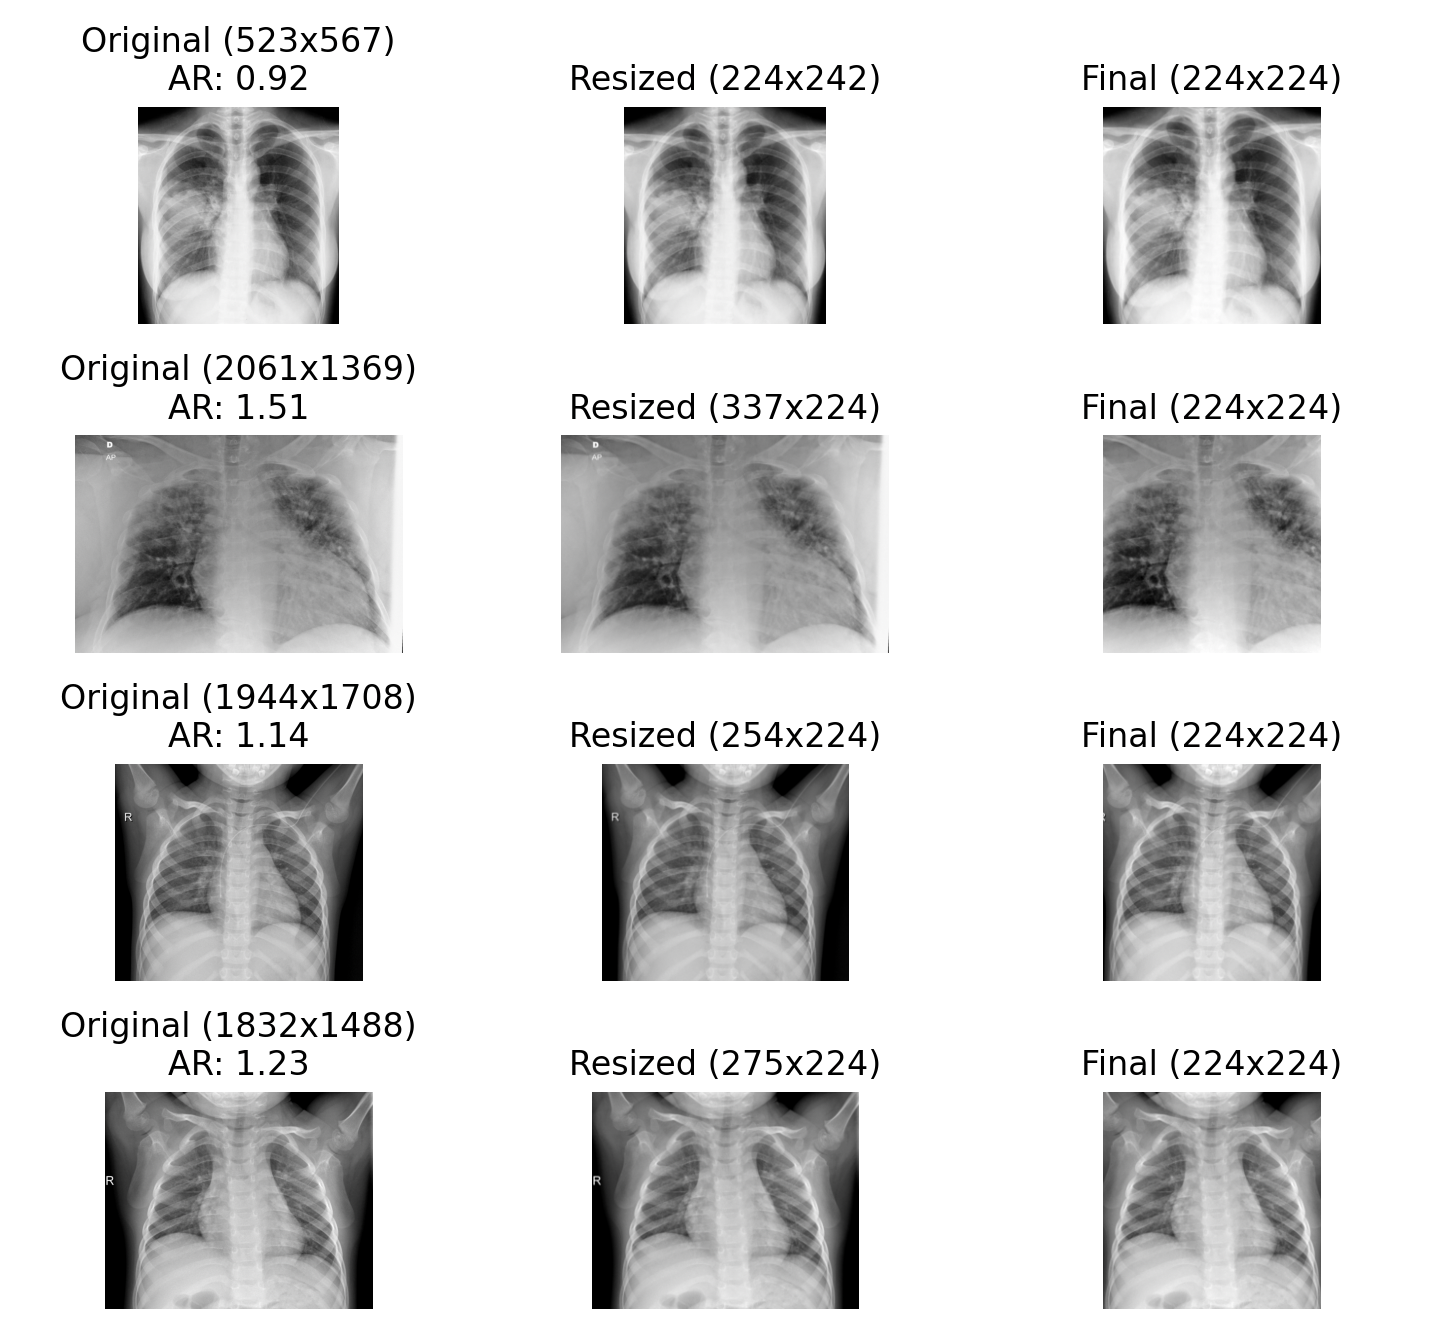
\includegraphics[width=1\textwidth]{transforms1.png}
        \caption{Ejemplo de preprocesamiento de imágenes.}
        \label{fig:preprocessing}
    \end{figure}

    \begin{figure}[H]
        \centering
        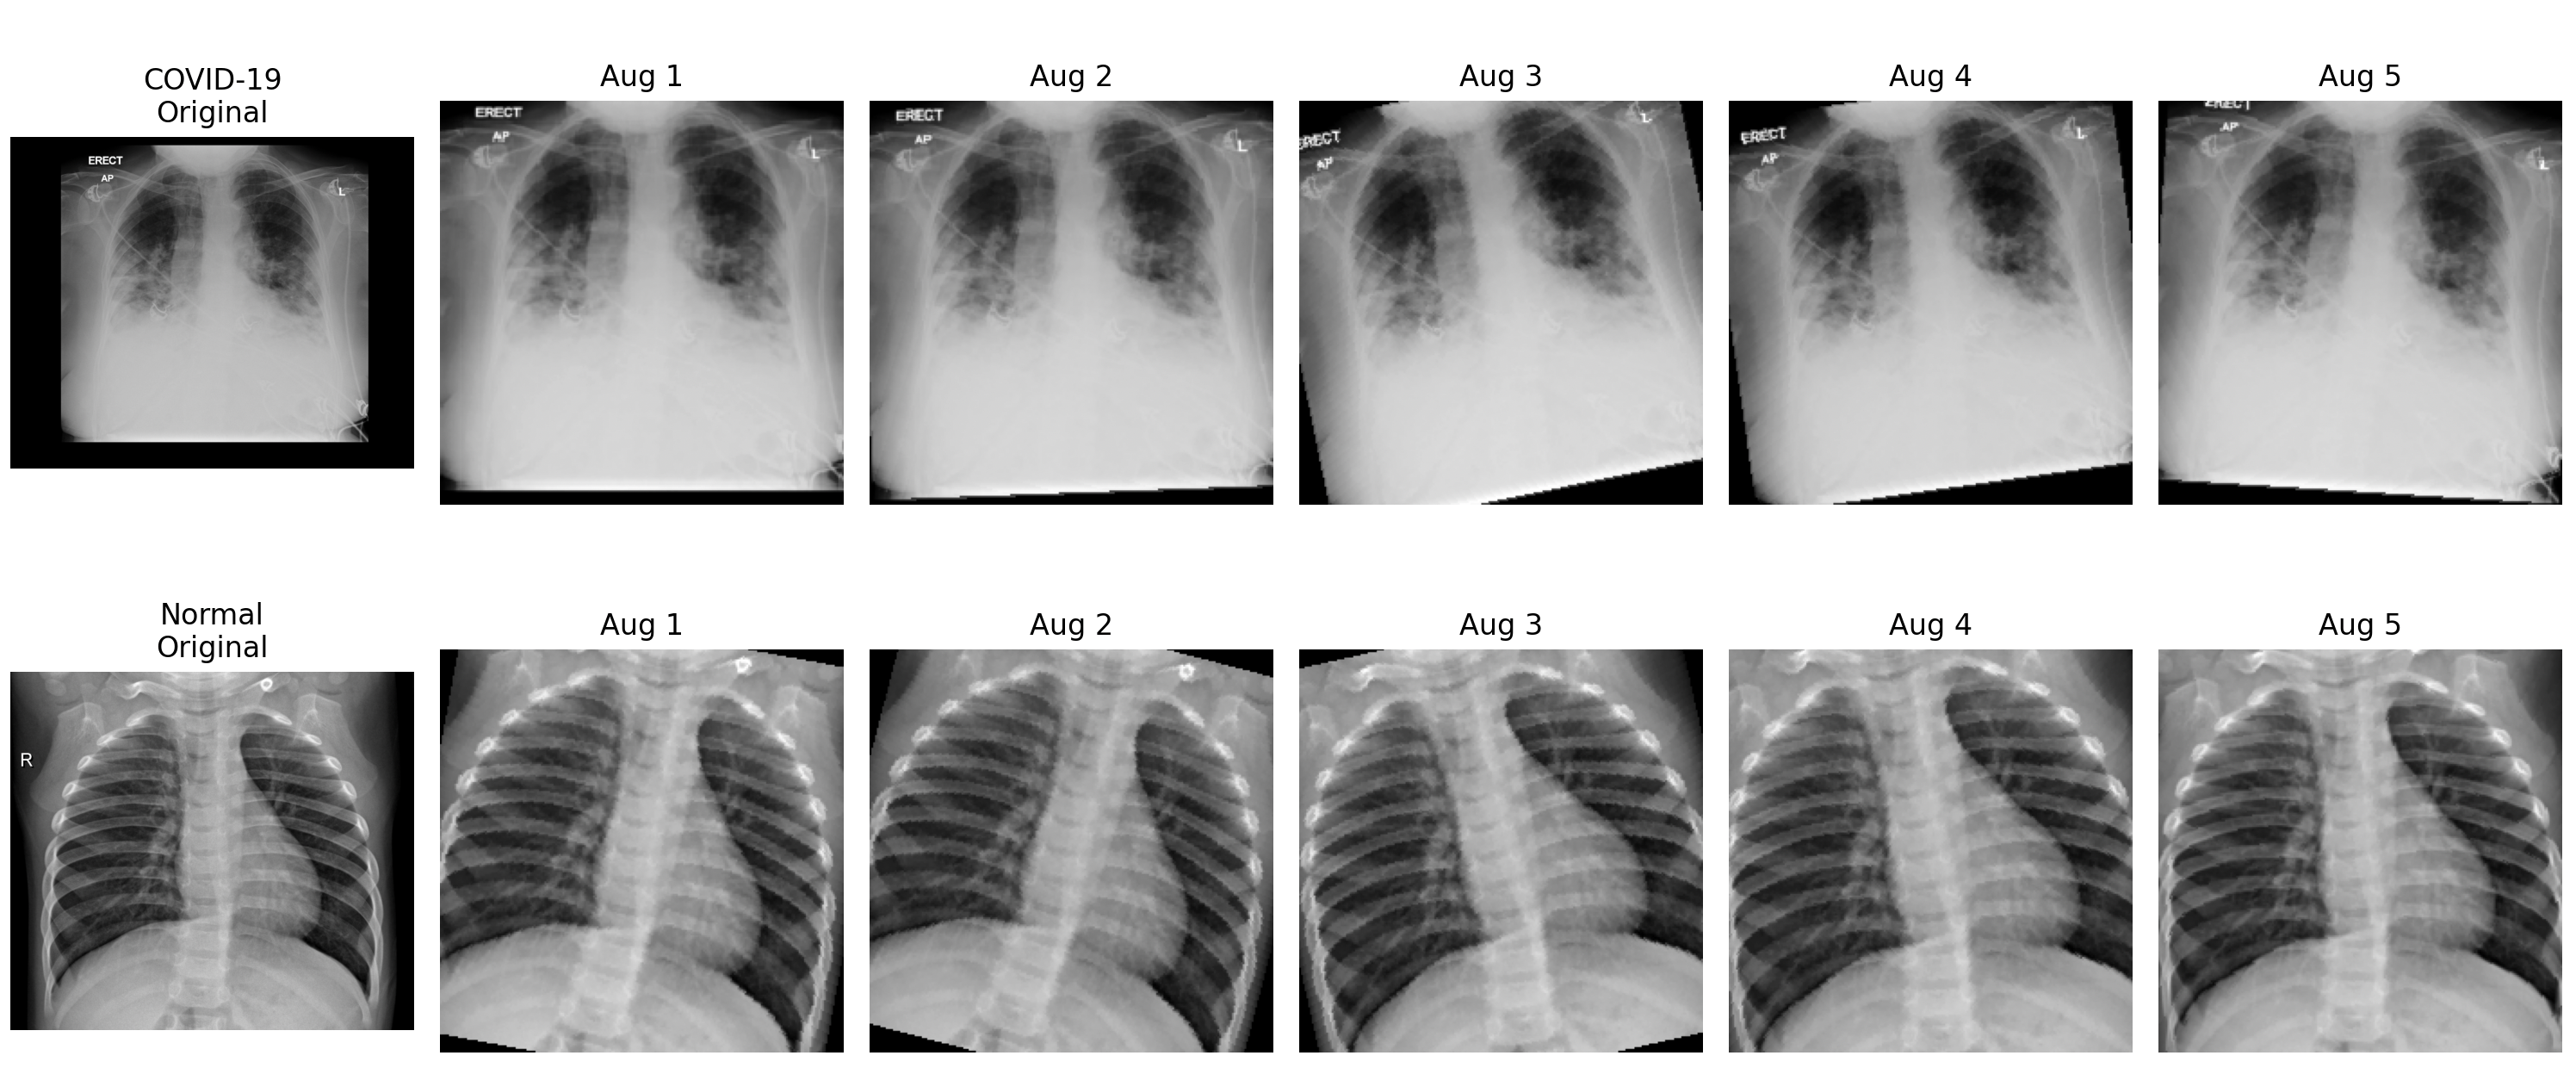
\includegraphics[width=1\textwidth]{transforms2.png}
        \caption{Ejemplo de aumentación de datos.}
        \label{fig:augmentation}
    \end{figure}
    
    \subsection{Tipo de clasificador}
    
    Después de experimentar con diversas arquitecturas, optamos por una Red Neuronal Convolucional (CNN) personalizada para nuestro clasificador. Este enfoque se basó en varios factores. Las pruebas iniciales con modelos preentrenados como DenseNet-169 y ResNet-18 mediante transfer learning revelaron que estos modelos eran excesivamente complejos para la tarea, lo que resultaba en un aprendizaje demasiado rápido y potenciales problemas de overfitting. Por tanto, decidimos implementar una CNN más simple y entrenarla desde cero para adaptarla mejor a las características del problema.
    
    \subsection{Arquitectura de la red}
    
    Nuestra CNN consta de los siguientes componentes:
    
    \begin{itemize}
        \item \textbf{Capas convolucionales}: Cinco bloques convolucionales, cada uno compuesto por:
        \begin{itemize}
            \item Una capa de convolución 2D con kernel de tamaño $3 \times 3$ y padding de 1
            \item Batch Normalization \cite{ioffe2015batchnormalizationacceleratingdeep} para estabilizar el aprendizaje
            \item Función de activación ReLU
            \item Max Pooling con kernel de tamaño $2 \times 2$ y stride de 2
        \end{itemize}
        
        \item \textbf{Canales de características}: La red aumenta progresivamente el número de filtros: $1 \rightarrow 32 \rightarrow 64 \rightarrow 128 \rightarrow 256 \rightarrow 256$
        
        \item \textbf{Clasificador}: Tras las capas convolucionales, incluimos:
        \begin{itemize}
            \item Aplanamiento (Flatten) de las características extraídas
            \item Una capa completamente conectada con 512 neuronas y activación ReLU
            \item Capa de Dropout con probabilidad de 5 para reducir el overfitting
            \item Capa de salida con 2 neuronas (una por clase)
        \end{itemize}
        
        \item \textbf{Función de pérdida}: Cross Entropy Loss, adecuada para problemas de clasificación multiclase
        
        \item \textbf{Regularización}: Además del Dropout mencionado, utilizamos Batch Normalization en cada bloque convolucional para estabilizar el entrenamiento y reducir el overfitting
    \end{itemize}
    
    \subsection{Estrategia de entrenamiento}
    
    Implementamos las siguientes estrategias para el entrenamiento de nuestro modelo:
    
    \begin{itemize}
        \item \textbf{Número máximo de epochs}: 30, con early stop basada en la métrica F1 del conjunto de validación
        \item \textbf{Tamaño de mini-batch}: 32 imágenes
        \item \textbf{Inicialización de pesos}: Inicialización aleatoria por defecto de PyTorch
        \item \textbf{Optimizador}: Adam con learning rate de 0.001
        \item \textbf{Parada temprana}: Implementamos un mecanismo de early stop con paciencia de 7 epochs y una delta mínima de 0.001 en la puntuación F1 de validación
        \item \textbf{División de datos}: 80\% para entrenamiento y 20\% para validación
    \end{itemize}

    Utilizamos Adam como optimizador debido a su capacidad para adaptarse a diferentes tasas de aprendizaje y su eficiencia en la convergencia frente a otros optimizadores más clásicos como SGD.
    
    \section{Implementación y recursos}
    
    \subsection{Hardware utilizado}
    
    El entrenamiento del modelo se realizó en un MacBook Pro de 14 pulgadas con las siguientes especificaciones:
    
    \begin{itemize}
        \item Procesador: Apple M3 Max 16 cores (12 performance and 4 efficiency). GPU de 40 cores.
        \item Memoria RAM unificada: 128 GB
        \item Aceleración por hardware: Metal Performance Shaders (MPS)
    \end{itemize}
    
    \section{Experimentos y resultados}
    
    \subsection{Proceso de experimentación}
    
    Nuestro proceso de experimentación siguió un enfoque iterativo:
    
    \begin{enumerate}
        \item \textbf{Transfer learning}: Evaluamos modelos preentrenados mediante transfer learning, concretamente DenseNet-169 y ResNet-18. Observamos que estos modelos convergían demasiado rápido, lo que sugería que eran excesivamente complejos para la tarea o que podían existir problemas en los datos.
        
        \item \textbf{Red personalizada}: Decidimos implementar una CNN personalizada más simple y entrenarla desde cero, lo que nos dio mayor control sobre la arquitectura y permitió ajustarla mejor a las características del problema. Sin embargo, también observamos un aprendizaje rápido, lo que nos llevó a sospechar de la calidad de los datos.
        
        \item \textbf{Fase de análisis}: Implementamos técnicas de interpretabilidad visual (GradCAM) para entender en qué regiones de la imagen se estaba centrando el modelo para tomar sus decisiones.
    \end{enumerate}
    
    \subsection{Tiempo de entrenamiento}
    
    El entrenamiento del modelo final se completó en 16 minutos y 19 segundos. El early stop se activó después de 27 epochs al no observarse mejoras significativas en la métrica F1 del conjunto de validación durante 7 epochs consecutivos.

    \begin{centering}
    \begin{figure}[H]
        \centering
        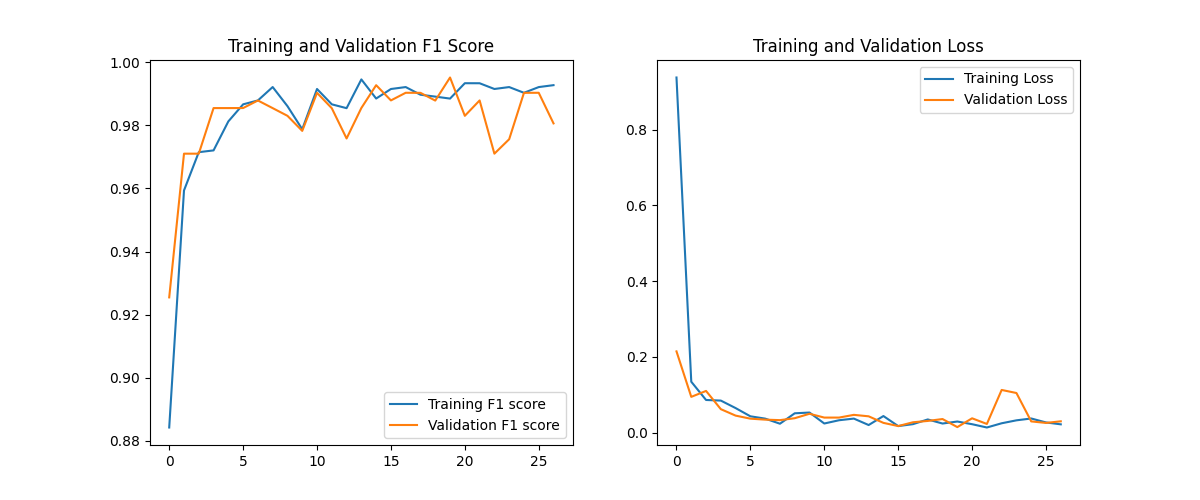
\includegraphics[width=1\textwidth]{training_history.png}
        \caption{Curvas de entrenamiento y validación del modelo.}
        \label{fig:training}
    \end{figure}
    \end{centering}

    \subsection{Análisis de contaminación de datos}
    
    Durante la evaluación de checkpoints intermedios, notamos que los resultados eran excepcionalmente altos, lo que nos llevó a investigar la calidad del conjunto de datos. A través de un análisis visual de las imágenes, descubrimos que en el conjunto de COVID-19, algúnas contenían anotaciones o marcas indicando la presencia de áreas de interés. 
    
    Ya que si limpiabamos estas imagenes con anotaciones el conjunto de COVID-19 se reduciría considerablemente, decidimos utilizar no el dataset reducido que se nos proporcionó, sino el dataset completo, que contiene un mayor número de imágenes. Sin embargo, este conjunto de datos también presentaba problemas de calidad. Por ejemplo, algunas imágenes estaban borrosas o mal alineadas, lo que podría afectar negativamente al rendimiento del modelo. Había imágenes con diferentes resoluciones y formatos, lo que complicaba el preprocesamiento y la normalización de los datos.
    Ademas, las radiografías del tórax estaban tomadas en dos posiciones diferentes (frontal y lateral), mientras que las del conjunto normal eran todas frontales. También había alguna imagen que no se trataba de una radiografía, sino de una resonancia magnética, que podría haber influido en el rendimiento del modelo.

    Viendo esto, decidimos hacer una limpieza del conjunto de datos, eliminando \textbf{manualmente} las imágenes contaminadas y aquellas que no cumplían con los criterios de calidad. Con estos cambios se redujo el número de imágenes del conjunto de COVID-19, pero aumentó la calidad del conjunto de datos. 
    
    \subsection{Resultados de clasificación}
    
    El modelo final obtuvo los siguientes resultados en el conjunto de validación:
    
    \begin{itemize}
        \item \textbf{Exactitud (Accuracy)}: 98\%
        \item \textbf{F1-Score}: 99.51\%
        \item \textbf{Área bajo la curva ROC (AUC-ROC)}: 0.9996
        \item \textbf{Sensibilidad (Recall para la clase COVID-19)}: 97.99\%
        \item \textbf{Matriz de confusión}:
    \end{itemize}
    
    \begin{center}
    \begin{tabular}{|c|c|c|}
        \hline
        & Predicho COVID-19 & Predicho Normal \\
        \hline
        Real COVID-19 & 244 & 5 \\
        \hline
        Real Normal & 3 & 160 \\
        \hline
    \end{tabular}
    \end{center}
    
    Estos resultados muestran un rendimiento excepcionalmente alto, con casi una clasificación perfecta, lo cual podría sugerir un posible overfitting o problemas en el conjunto de datos.
    
    \subsection{Análisis de interpretabilidad (GradCAM)}
    Dado que tras el análisis de los resultados iniciales y la limpieza del conjunto de datos, el modelo parecía aprender patrones no deseados, decidimos implementar técnicas de interpretabilidad para comprender mejor su comportamiento. En este caso, utilizamos GradCAM, que nos permite visualizar las regiones de la imagen que más influyen en la decisión del clasificador.

    \begin{figure}[H]
        \centering
        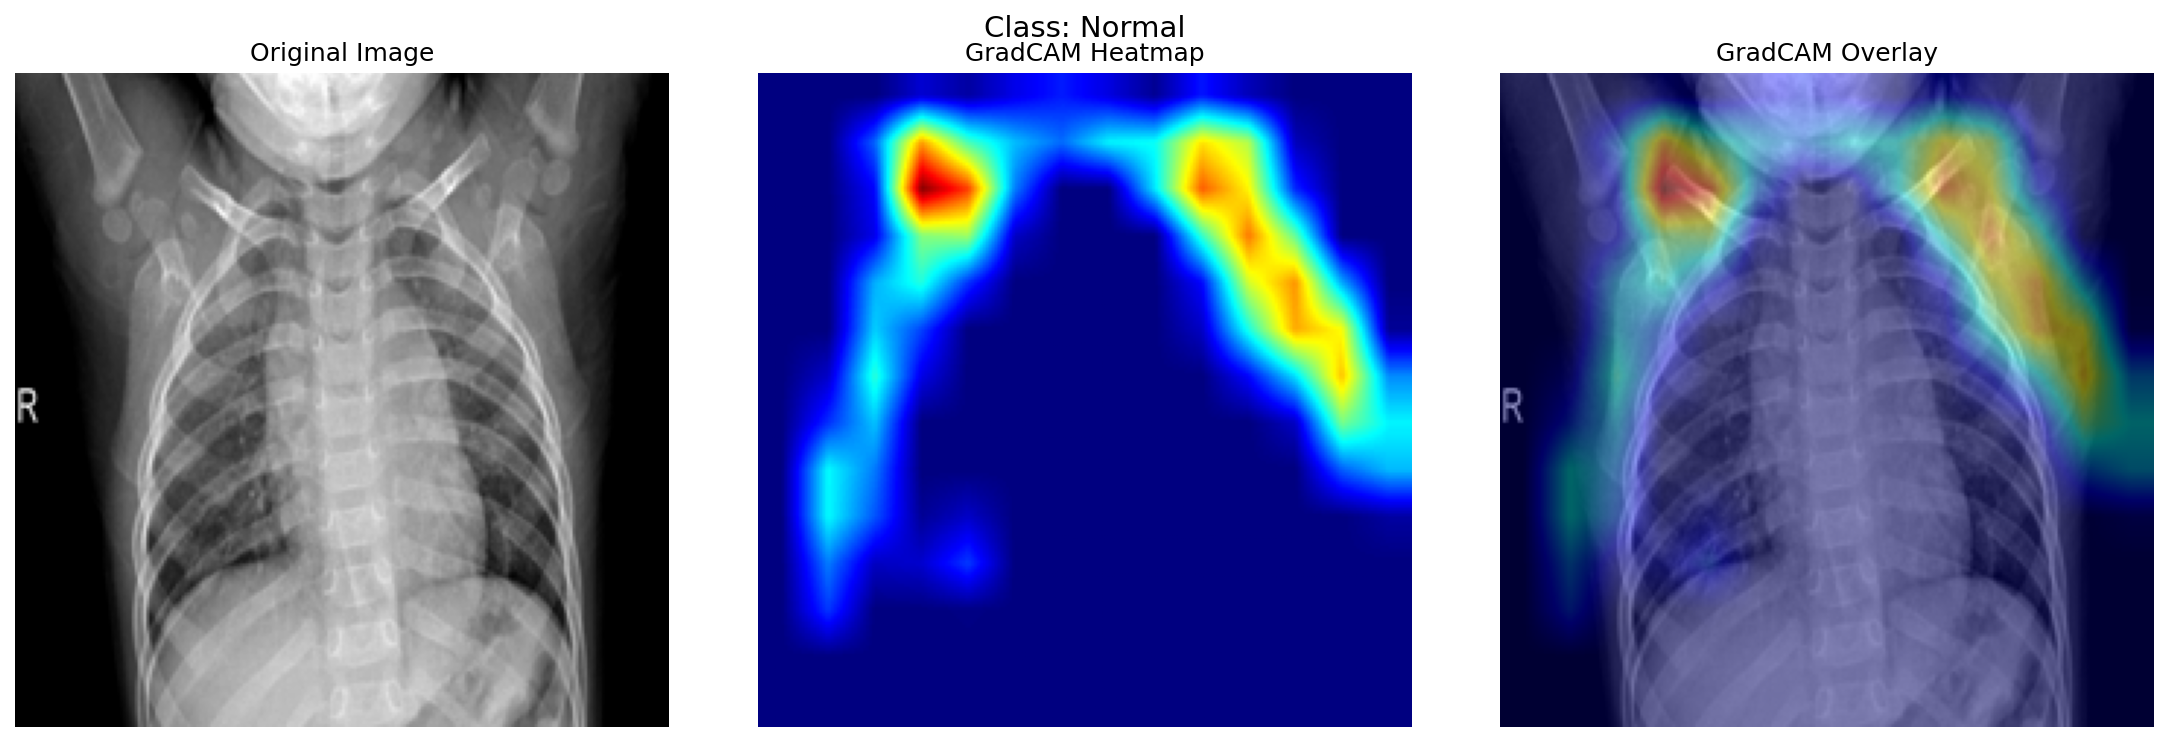
\includegraphics[width=1\textwidth]{NORMAL2-IM-0932-0001_gradcam.png}
        \caption{Ejemplo de visualización GradCAM en una imagen de rayos X (Clase Normal).}
        \label{fig:gradcam}
    \end{figure}
    En la figura \ref{fig:gradcam} se muestra un ejemplo de la visualización GradCAM aplicada a una imagen normal. La región resaltada en rojo indica la zona de la imagen que el modelo considera más relevante para su decisión. En este caso, el modelo parece centrarse en el área del brazo del paciente, lo que no tiene relación con la patología que se busca clasificar.

    Tras analizar varias imágenes, observamos que el modelo tiende a enfocarse en áreas no relevantes, como los brazos de los pacientes o marcas en las radiografías. Esto refuerza la hipótesis de que el modelo ha aprendido patrones no deseados debido a la contaminación del conjunto de datos.

    Haciendo un análisis más profundo, nos percatamos de otro problema: en el conjunto de COVID-19, los pacientes tenían los brazos hacia abajo, mientras que en el conjunto normal, los brazos estaban hacia arriba. Esto llevó al modelo a aprender a clasificar las imágenes en función de la posición de los brazos, en lugar de la presencia de COVID-19.

    \section{Modelo Multiclase}
    Dado que el conjunto de datos estaba contaminado y el modelo no estaba aprendiendo a clasificar correctamente las imágenes, decidimos no continuar con el modelo de clasificación multiclase, que incluía además de COVID-19 y normal, la clase de neumoía bacteriana. Los resultados obtenidos en el modelo binario no eran confiables, por lo que no tenía sentido continuar con un modelo más complejo. Sin embargo, si se hubiera continuado, el modelo multiclase habría seguido la misma arquitectura y metodología que el modelo binario, pero con una capa de salida de 3 neuronas y una función de activación softmax.

    \section{Conclusiones}
    
    El clasificador de COVID-19 basado en imágenes de rayos X desarrollado en este trabajo muestra un rendimiento aparentemente excepcional, pero este resultado extremadamente positivo debe interpretarse con cautela por varios motivos.
    
    El análisis de interpretabilidad mediante GradCAM y el estudio detallado del conjunto de datos reveló problemas de contaminación en los datos, lo que significa que el modelo aprendió patrones artificiales o marcas no relacionadas con la patología. Asimismo, el hecho de que modelos complejos como DenseNet-169 y ResNet-18 aprendieran demasiado rápido fue una señal temprana de posibles problemas con el conjunto de datos. A pesar de las métricas casi perfectas, la utilidad clínica real de este modelo es nula debido a los problemas identificados.
    
    Como bien se dice en el deep learning, los datos son lo más importante. Al tener un conjunto de datos contaminado, el modelo aprendió no a indentificar la presencia de COVID-19, sino a identificar la posición de los brazos de los pacientes. También destaca el valor de las técnicas de interpretabilidad como GradCAM, que nos permiten no solo evaluar el rendimiento numérico de un modelo, sino también comprender su comportamiento y detectar posibles fallos o sesgos en su proceso de toma de decisiones. Gracias a estas técnicas, pudimos identificar que el modelo no estaba aprendiendo a clasificar las imágenes en base a la presencia de la patología, sino de características irrelevantes como la posición de los brazos de los pacientes o marcas en las radiografías. 

    \subsection{Trabajos futuros}
    Para futuros trabajos, sería recomendable realizar un análisis más exhaustivo del conjunto de datos antes de entrenar el modelo. En nuestro trabajo, la limpieza del conjunto de datos se realizó de manera manual, lo que puede ser poco eficiente y propenso a errores. Una opción sería implementar un proceso automatizado para detectar y eliminar imágenes contaminadas o de baja calidad. Un posible enfoque sería utilizar técnicas de segmentación de imágenes \cite{ravi2024sam2segmentimages} \cite{Tartaglione_2020} para filtrar únicamente las regiones relevantes de las radiografías, eliminando áreas no relacionadas con la patología. 

    Además, sería interesante explorar el uso de técnicas de data augmentation más avanzadas, como la generación de imágenes sintéticas mediante GANs (Generative Adversarial Networks) \cite{goodfellow2014generativeadversarialnetworks}, para aumentar la diversidad del conjunto de datos y mejorar la capacidad de generalización del modelo. Utilizando esta técnica, podríamos generar imágenes de rayos X sintéticas que simulen diferentes condiciones patológicas a partir de radiografías reales, lo que podría enriquecer el conjunto de datos y ayudar al modelo a aprender patrones más robustos.

    Otra opción sería utilizar GPTs (Generative Pre-trained Transformers) multimodales para realizar la clasificación de imágenes. Estos modelos han demostrado un rendimiento excepcional en tareas de clasificación y segmentación de imágenes, y podrían ser una alternativa interesante a las CNN tradicionales. Sin embargo, su implementación es más compleja y requiere un mayor esfuerzo computacional. Uno de estos modelos es Qwen2.5-VL, que ha demostrado un rendimiento sobresaliente en tareas de clasificación y segmentación de imágenes \cite{bai2025qwen25vltechnicalreport}.

  \end{report}


  % bibliography
   \label{bibliography}
   \part{Bibliografía}
   \printbibliography[heading=none]  % alternative

  % appendices
%   \begin{appendices}
%     \part{Apéndices}  % optional
%     \section{Mi apéndice}

%   \end{appendices}

\end{document}
